In their work \cite{boson}, Aaronson and Arkhipov introduced a quantum computation model in which a number of identical photons (which are considered boson particles) pass through a \textbf{linear optical network} and are then counted at the end of the network using photonic detectors, as shown in Fig. \ref{fig:bosonsample}. They provide evidence that computations relying on optical quantum elements cannot be efficiently simulated by classical computers. This feature makes it a good foundation to create a True Random Number Generator using this model as an entropy source.

\begin{figure}
\centering
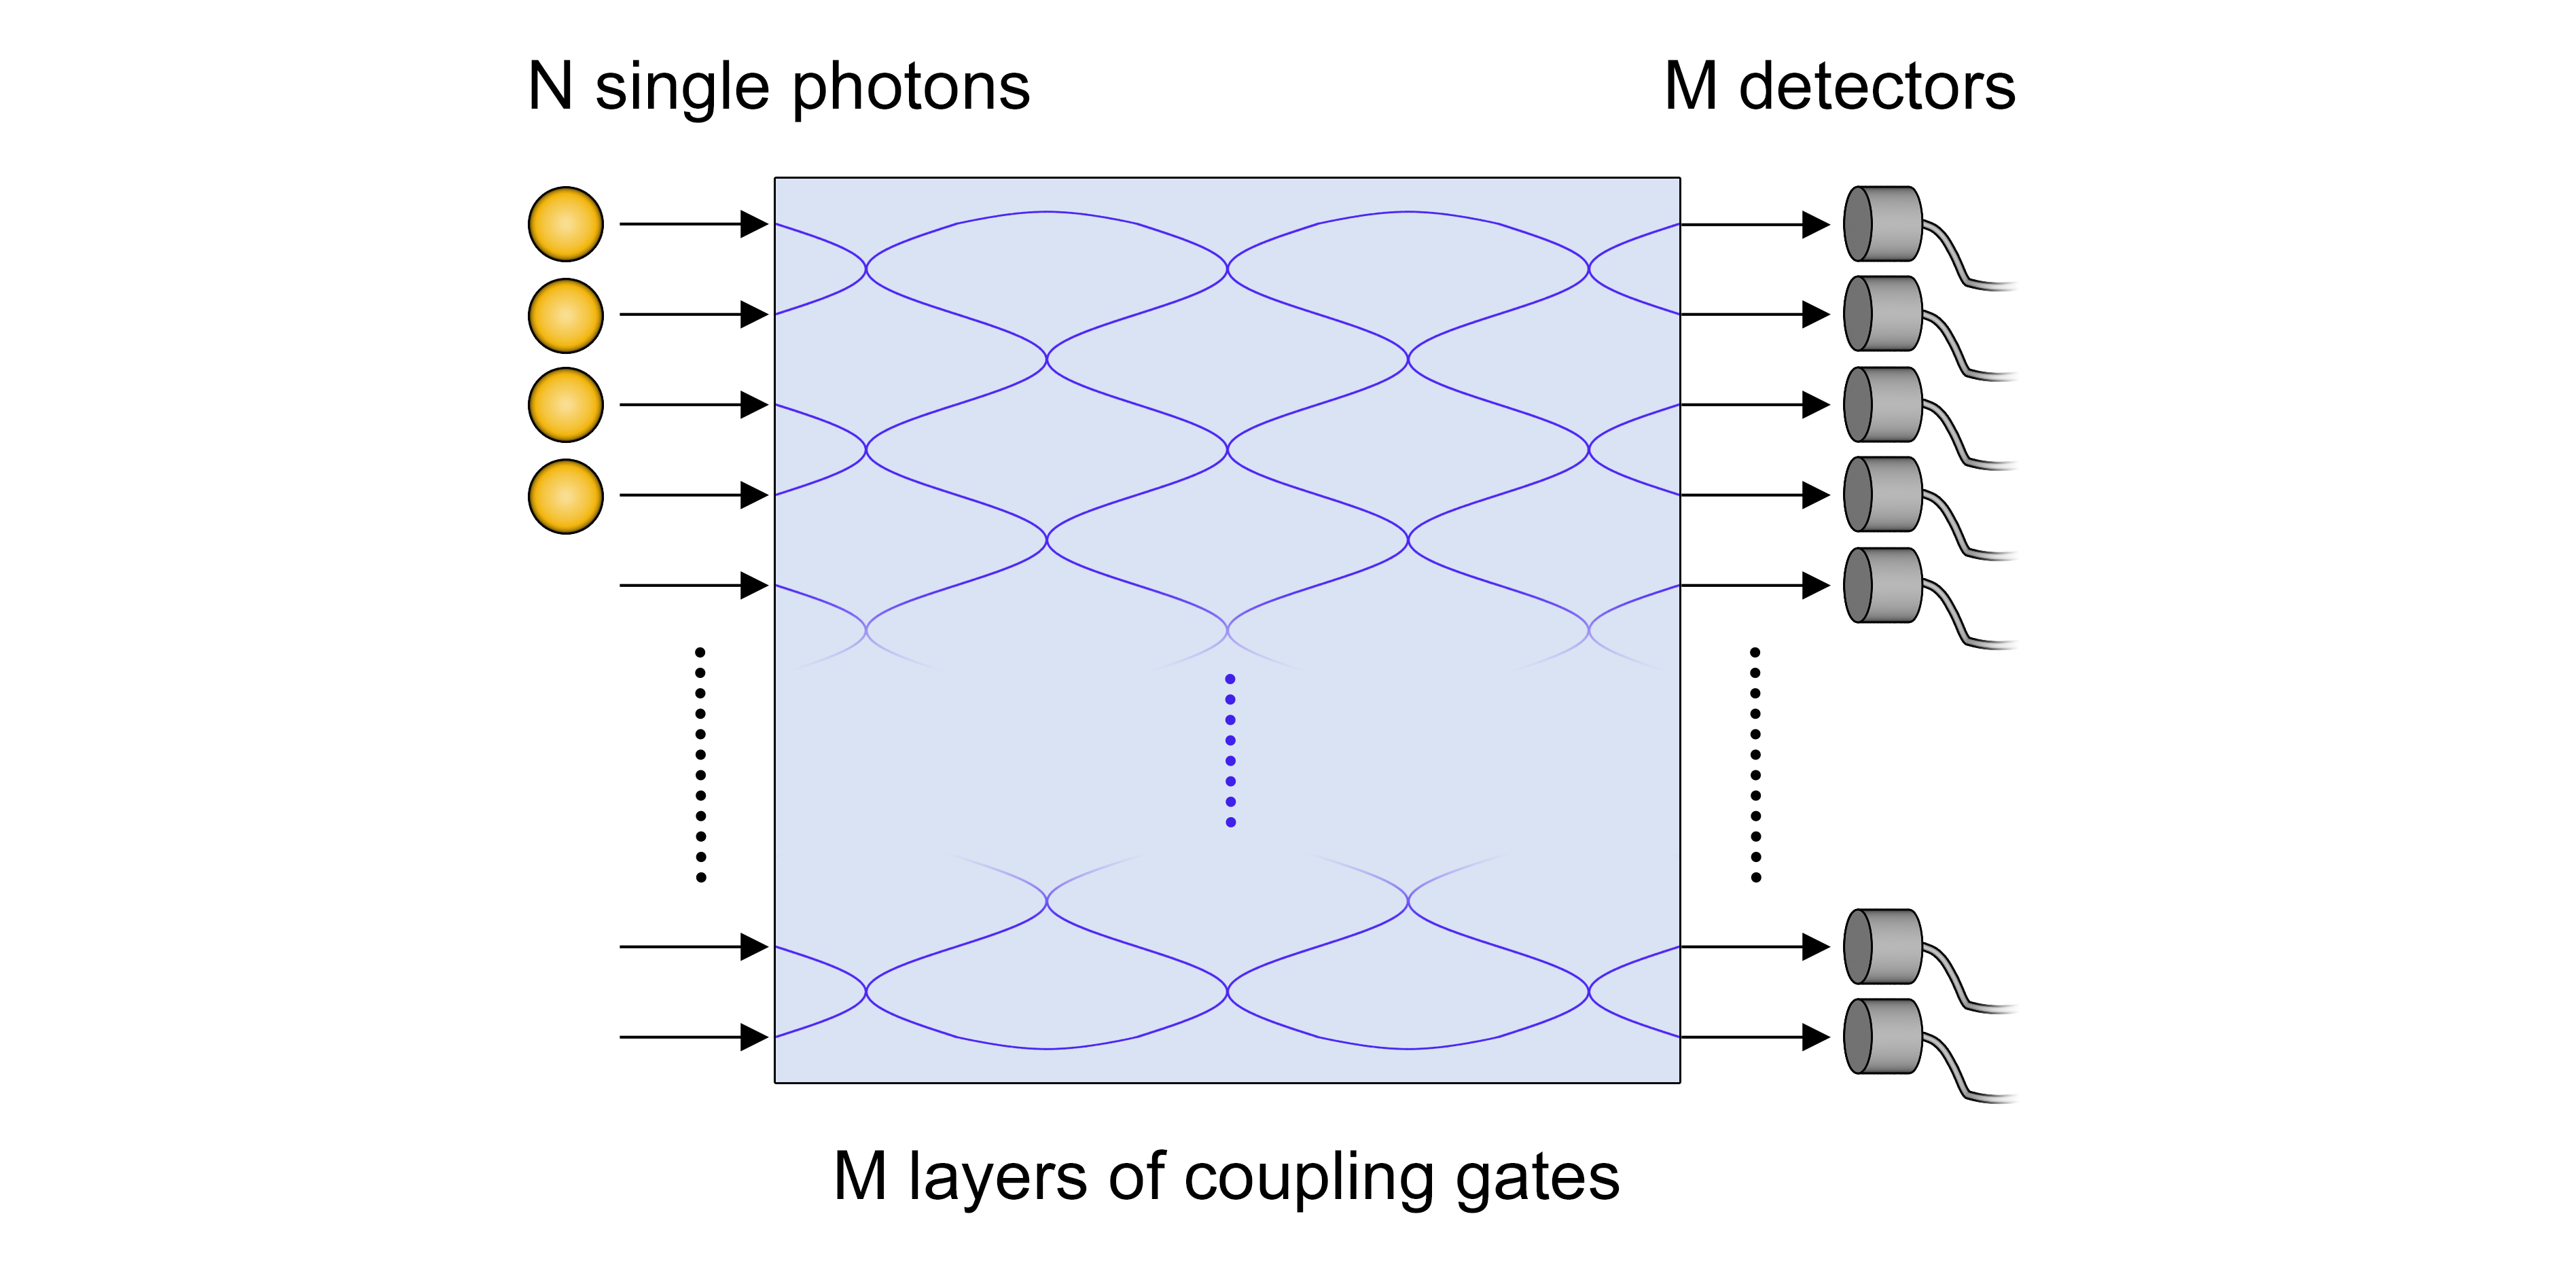
\includegraphics[width=16cm]{figures/1712.10037v3.png}\vspace{-0.2cm}
\caption{In a boson sampling device N single photons are sent over an M mode linear optical circuit composed of M layers of two-mode coupling gates and detected at the output with photon counting detectors. \cite{dede}}
\label{fig:bosonsample}
\end{figure}

\section{Preliminaries}
\subsection{The Fock States and the Fock Space}
Consider a quantum system where we have multiple identical quantum particles, each occupying a state within a Hilbert space. We want to study the entire multi-particle system and its states.

For example, if we have a system that contains two bosonic particles, where each of their states is described by a wave function \( |\psi_1\rangle \) and \( |\psi_2\rangle \) in the Hilbert space, then the entire state of the system (constructed from boson 1 and boson 2 respectively) can be described as the tensor product of these two states:

\begin{equation}
|\psi_{1,2}\rangle = |\psi_1\rangle \otimes |\psi_2\rangle
\end{equation}

However, if the two particles are identical bosons, we cannot distinguish which particle is in which state anymore. This means that for the multi-particle system, there should be an equal probability of finding particle 1 in state \( x_1 \) and particle 2 in state \( x_2 \), and vice versa. Therefore:

\begin{equation}
|\psi_{12}\rangle = |\psi_1\rangle \otimes |\psi_2\rangle
\end{equation}

should be equal to finding particle 2 in state \( x_2 \) and particle 1 in state \( x_1 \):

\begin{equation}
|\psi_{21}\rangle = |\psi_2\rangle \otimes |\psi_1\rangle
\end{equation}

Thus, we have:

\begin{equation}
|\psi_{12}\rangle = |\psi_{21}\rangle
\end{equation}

Introducing this symmetry should be ensured in the multi-particle system:

\begin{equation}
|\psi\rangle = \frac{1}{\sqrt{2}} \left( |\psi_1\rangle \otimes |\psi_2\rangle + |\psi_2\rangle \otimes |\psi_1\rangle \right)
\end{equation}

Here, the Fock space comes into play to introduce the second quantization representation, which focuses on the number of particles in each possible state, rather than which particle occupies which state (as in the first quantization representation).

A \textbf{Fock state} \( |F\rangle \) represents the infinite occupation numbers of particles in \textbf{all possible state of the Hilbert space} \( |u_i\rangle \). The occupation number \( n_i \) corresponds to the number of particles occupying the \( i \)-th quantum state \( |u_i\rangle \).

For example, if the state \( |u_1\rangle \) is occupied by \( n_1 \) particles, the Fock state can be written as:

\begin{equation}
|F\rangle = |n_1, n_2, \dots, n_i, \dots \rangle
\end{equation}

where \( n_1, n_2, \dots \) are the occupation numbers for the respective quantum states \( |u_1\rangle, |u_2\rangle, \dots \). In the case of bosons, the occupation numbers \( n_i \) can take any non-negative integer value, representing the number of bosons occupying each state.



\subsection{The Permanent of a Matrix}

The permanent is a function applied only to square matrices. It is calculated similarly to the determinant but without taking into consideration the sign of the matrix elements (all terms are considered positive). The formula for the permanent of an \( n \times n \) matrix \( A = [a_{ij}] \) is:

\begin{equation}
\text{perm}(A) = \sum_{\sigma \in S_n} \prod_{i=1}^{n} a_{i,\sigma(i)}
\end{equation}

where \( S_n \) is the set of all permutations of \( \{1, 2, \dots, n\} \), and \( \sigma \) represents a permutation.

\subsection{The Haar Unitary Matrix}

A Haar unitary matrix is a random unitary matrix generated from the Haar measure, which is defined as the only uniformly distributed group of unitary matrices. Generating a Haar unitary matrix means producing a random matrix that remains unitary.


\section{The Uncertainty of the Boson Sampling Quantum System}

Shi et al. in \cite{shi_Twa3na} designed a Quantum Random Number Generator (QRNG) based on boson sampling, exploiting its inherent randomness to output true random numbers.

In this system, \( N \)-photons represented by Fock states are introduced into a randomly configured optical network of beam splitters and interferometers, modeled by a Haar unitary matrix \( U \). The output state (also expressed in Fock states) \( \ket{\psi_{\text{out}}} \) represents the probability of detecting \( j_i \) photons by the \( i \)-th detector. This probability can be calculated using the following formula:


\begin{equation}
    P(\mathbf{j}) = \frac{\left| \operatorname{Perm}(U_{\mathbf{j}}) \right|^2}{\prod_{i=1}^{m} j_i!}
\end{equation}





where \( \operatorname{Perm}(U_{\mathbf{j}}) \) is the permanent of the submatrix \( U_{\mathbf{j}} \) corresponding to the input and output modes, and \( \mathbf{j} = (j_1, j_2, \dots, j_m) \) is the output configuration with \( j_i \) photons detected at the \( i \)-th mode.

Shi et al. used single-photon detectors, which are easier to implement physically. Each detector collects whether there is a photon at that mode (or multiple photons) or not, providing the bitstring representation needed for random number generation.

The output of this boson sampling system is a superposition of all possible Fock states:


\begin{equation}
    \ket{\psi_{\text{out}}} = \sum_i \lambda_i \ket{\psi_i}

\end{equation}    



According to the fundamental randomness of quantum mechanics, when the final state is measured using the detectors, the system collapses randomly to one of the possible states with a probability proportional to the square of the corresponding coefficient \( |\lambda_i|^2 \). Since the bosonic state evolves through beam splitters and interferometers, this randomness increases, making the boson sampling output more suitable as an entropy source for a true random number generator.


\section{The Unreproducibility of the Boson Sampling Quantum System}

The results of the boson sampler are completely independent of the initial input state. The initial input configuration does not affect the output, as the system evolves through a Haar unitary matrix \( U \), representing the randomness introduced by beam splitters and interferometers.

As stated by Shi et al. in \cite{shi_Twa3na}, boson sampling QRNGs cannot be efficiently simulated as the output size increases. This is due to the computational complexity of calculating the \textbf{permanent of a matrix}, which grows exponentially with the system size. The permanent calculation is essential in describing the system's evolution, making classical simulation infeasible for large-scale boson sampling systems.



